\documentclass[UTF8]{ctexart}
\usepackage{graphicx}
\usepackage{float}
\usepackage{geometry}
\usepackage{fancyhdr}
\usepackage{lastpage}
\usepackage{amsmath}
\usepackage{mathrsfs}
\usepackage{amsthm}
\usepackage{multicol}
\usepackage{multirow}
\usepackage{booktabs}
\usepackage{subfigure}
\usepackage[colorlinks,linkcolor=black]{hyperref}
\geometry{left=2.54cm,right=2.54cm,top=3.18cm,bottom=3.18cm}%页边距
\pagestyle{fancy}
\lhead{
\includegraphics[scale=1]{sjtu-logo-red.pdf}}  
\rhead{CT成像的扫描与重建算法实现} 
\cfoot{第 \thepage\ 页\ 共 \pageref{LastPage} 页} 
\newtheorem{theorem}{定理}

\begin{document}

\begin{titlepage}
    \begin{center}
        
\includegraphics[width=0.8\textwidth]{sjtu-name-blue.pdf}\\[1cm]
        \textsc{\Huge \bfseries 课程报告}\\[1.5cm]
        
\includegraphics[width=0.3\textwidth]{sjtu-badge-blue.pdf}\\[0.5cm]    

        \Huge \bfseries{CT成像的扫描与重建算法实现}\\[1cm]
        \LARGE \bfseries{生物医学图像处理(2)课程作业}\\[1cm]
        \Large \bfseries{518021910971 裴奕博}
    \end{center}
\end{titlepage}
\tableofcontents
\newpage

%正文
\section{项目背景}

\subsection{CT重建算法}
自20世纪70年代被发明以来,X射线计算机断层成像(CT)在医学影像检查中扮演了越来越重要的地位。在CT成像的流程中,将图像进行数字化、投影和重建的算法非常重要。CT成像算法的好坏,会直接影响到CT的成像质量。

\subsection{数学基础}
中心切片定理和滤波反投影算法的提出,是CT成像和重建算法的数学基础。

中心切片定理可以表述如下:
\begin{theorem}[中心切片定理]
    $$P(\omega,\theta)=F(\omega\cos\theta,\omega\sin\theta)$$
    其中P是投影函数$p(l,\theta)$的傅里叶变换,$F(u,v)$是图像的
    二维傅里叶变换。
\end{theorem}
该定理说明,某断层在角度为$\theta$时得到的平行投影的一维傅里叶变换,等于图像二维傅里叶变换过原点的一个垂直切片,且切片的方向也为$\theta$角。\cite{ramesh1989algorithm}

通过中心切片定理,我们可以得到原CT图像的投影图,再经过重建算法就可以得到CT重建图像。重建算法主要分为两大类:滤波反投影算法和反卷积反投影算法。本次的重建算法属于滤波反投影算法,可以用公式表示如下:\cite{kak2002principles}

\begin{theorem}[滤波反投影算法]
    $$f(x,y)=\int_0^{\pi}|\omega|P(\omega,\theta)\exp(j2\pi\omega l)\lvert_{l=x\cos\theta+y\sin\theta}$$
\end{theorem}
其中$P(\omega,\theta)$是通过中心切片定理得到的投影图的傅里叶变换。
\newpage
\section{项目实现}
\subsection{项目总体实现}
项目的整体流程比较简单,如下图:

\begin{figure}[H]
    \centering
    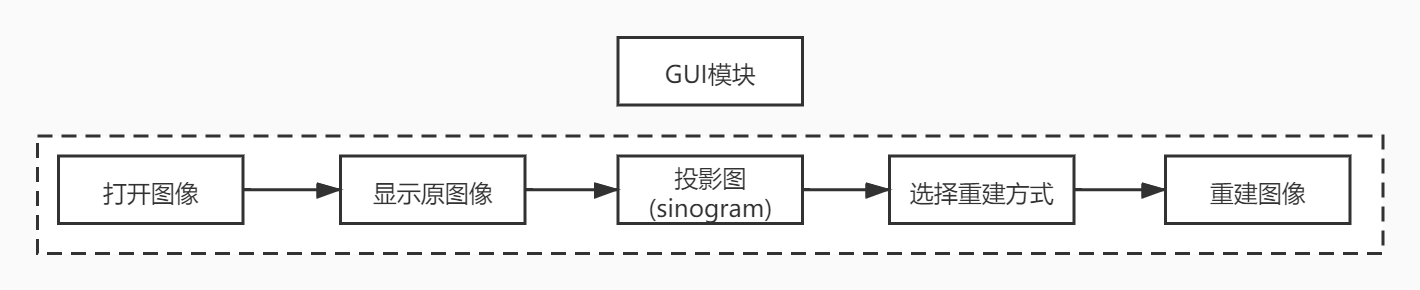
\includegraphics[width=\textwidth]{../image/workflow.jpg}
    \caption{项目流程图}
    \label{fig workflow}
\end{figure}
所有程序均采用Python实现,图形化界面使用PySide2图形化框架实现。图像处理与重建的部分使用numpy实现,所使用的的依赖包可见requirements.txt文件。

\subsection{Radon正变换的实现}
Radon正变换的实现方法如下图:
\begin{figure}[H]
    \centering
    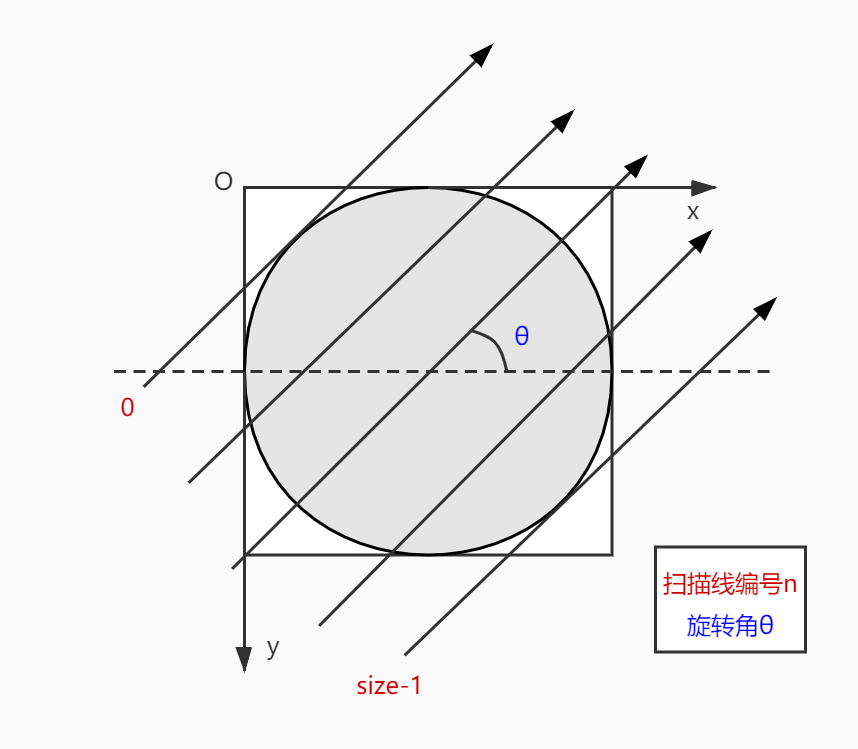
\includegraphics[width=0.6\textwidth]{../image/radon.jpg}
    \caption{Radon正变换实现}
    \label{fig Radon}
\end{figure}
其中最大的正方形表示待扫描的图像。我们默认扫描的区域范围用灰色部分显示。默认的扫描线方向如图中虚线所示,编号从上到下为$[0,size-1]$。扫描线与默认方向之间的夹角为$\theta$。设扫描点的坐标为$(x,y)$,图像中心点坐标为$(c,c)$,变换后的扫描点坐标为$P^\prime(x^\prime,y^\prime)$,使用齐次变换矩阵,有
% TODO 数学推导
\begin{equation}
    P^\prime=R(P-C)+C
\end{equation}
\begin{equation}
    \left[
        \begin{array}{c}
           x^\prime \\
           y^\prime \\
           1
        \end{array}
        \right]=
    \left[
        \begin{array}{ccc}
            \cos{\theta} & \sin{\theta} & 0\\
            -\sin{\theta} & \cos{\theta} & 0\\
            0 & 0 & 1
         \end{array}
    \right]
    \left[
        \begin{array}{c}
            x-c\\
            y-c\\
            0
        \end{array}
    \right]+\left[
        \begin{array}{c}
            c\\
            c\\
            1
        \end{array}
    \right]=
    \left[
        \begin{array}{ccc}
            \cos{\theta} & \sin{\theta} & c(1-\cos{\theta}- \sin{\theta})\\
            -\sin{\theta} & \cos{\theta} & c(1-\cos{\theta}+\sin{\theta})\\
            0 & 0 & 1
         \end{array}
    \right]
    \left[
        \begin{array}{c}
            x\\
            y\\
            1
        \end{array}
    \right]
\end{equation}
记上式为
\begin{equation}
    P^\prime=R\prime P
\end{equation}
即通过左乘R即可完成变换。由于Numpy对矩阵运算作了优化,因此直接进行矩阵运算相比逐项计算大大提升了速度。

最后将每条扫描线上的值相加,就可以得到其中一个$\theta$角所对应的扫描值,将其显示出来即可得到正弦图,上述所有过程均使用Numpy的矩阵运算来实现。

\subsection{Radon逆变换的实现}

Radon逆变换的实现比较简单,可分为三个部分:频域滤波、插值重建和后处理。
\begin{itemize}
    \item 频域滤波部分的FFT算法直接调用Scipy中的fft,ifft函数实现,部分滤波器也采用Numpy的相关滤波器函数实现。
    \item 插值重建部分采用了Scipy中的interp1d进行一维插值,默认使用线性插值法。
    \item 后处理部分:由于扫描时只扫描了中间圆形的部分,因此需要对圆形之外的区域置0,同时也要对负值进行一些处理。
\end{itemize}

\subsection{图形化界面的实现}

图形化界面采用了PySide2(PyQt)框架实现。UI文件储存在ui文件夹下,由两个页面组成,一个主页面和一个滤波反投影算法的参数选择界面。

\begin{figure}[H]
    \centering
    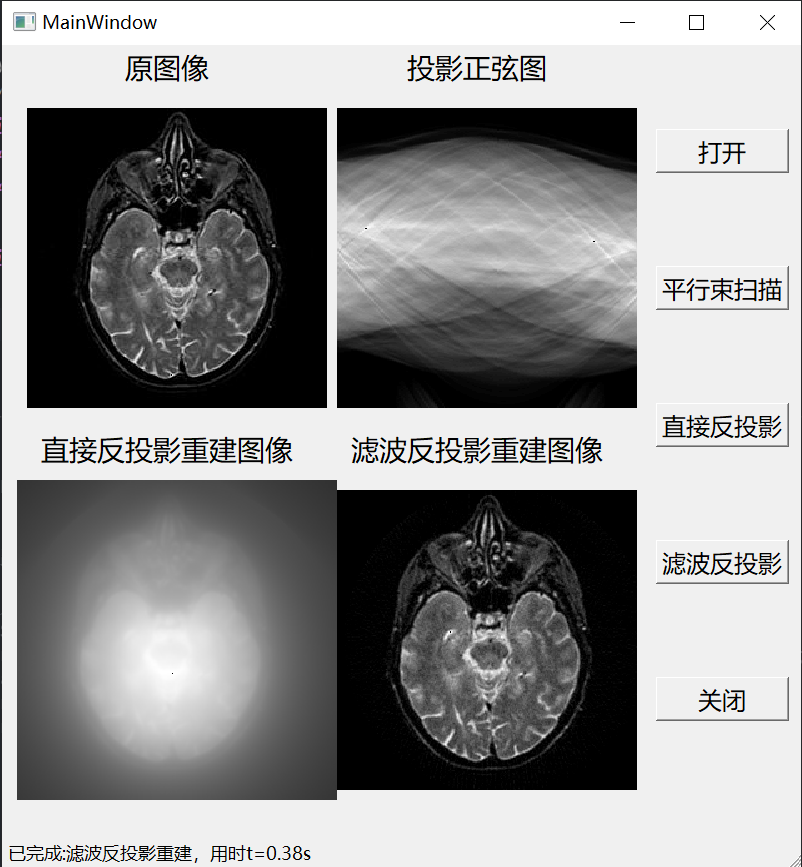
\includegraphics[width=0.7\textwidth]{../image/main_UI.png}
    \caption{主界面}
    \label{fig UI}
\end{figure}

本次实现的图形化界面具有以下几个特点:
\begin{itemize}
    \item 可以自行选择本地文件打开。
    \item 使用了多线程操作。图像处理等耗时的操作运行在另一个线程下,但是在计算过程中将页面上所有交互按钮禁用,防止用户进行误操作。
    \item 底部有状态栏,在运行过程中可以给予提示,运行结束后可以显示进行的操作和所消耗的时间。
    \item 在用户误操作时可以跳出错误提示。
\end{itemize}
\newpage
\section{项目结果和评价}
\subsection{可视化结果}
运行visualize.py,可以查看可视化结果如下:图\ref{fig result1}是shepp-logan模型的可视化结果,图\ref{fig result2}是使用CT图像test.jpg的可视化结果,两者均为256*26尺寸。每张结果图中,上面一行是本次实现的算法结果,下面一行是skimage库中radon和iradon变换实现的结果。
\begin{figure}[H]
    \centering
    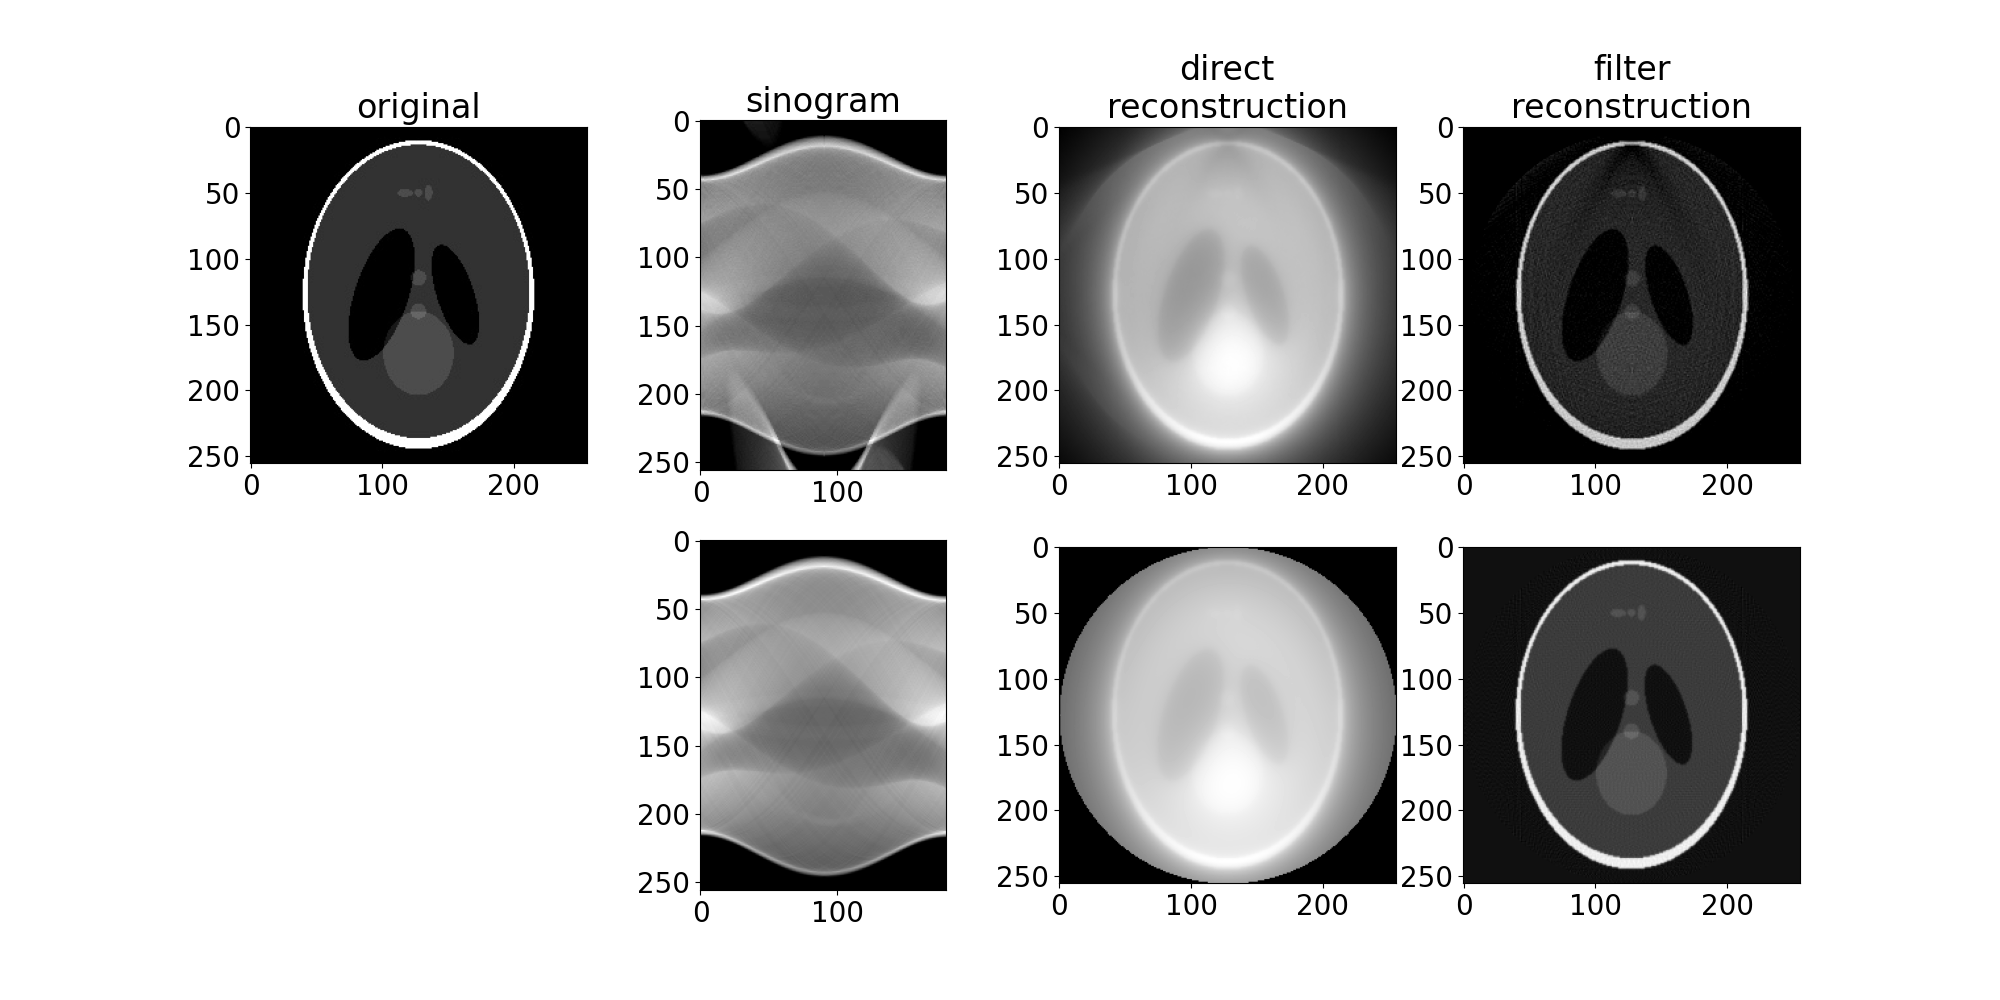
\includegraphics[width=0.9\textwidth]{../image/sl_model.png}
    \caption{shepp-logan模型重建结果}
    \label{fig result1}
\end{figure}


\begin{figure}[H]
    \centering
    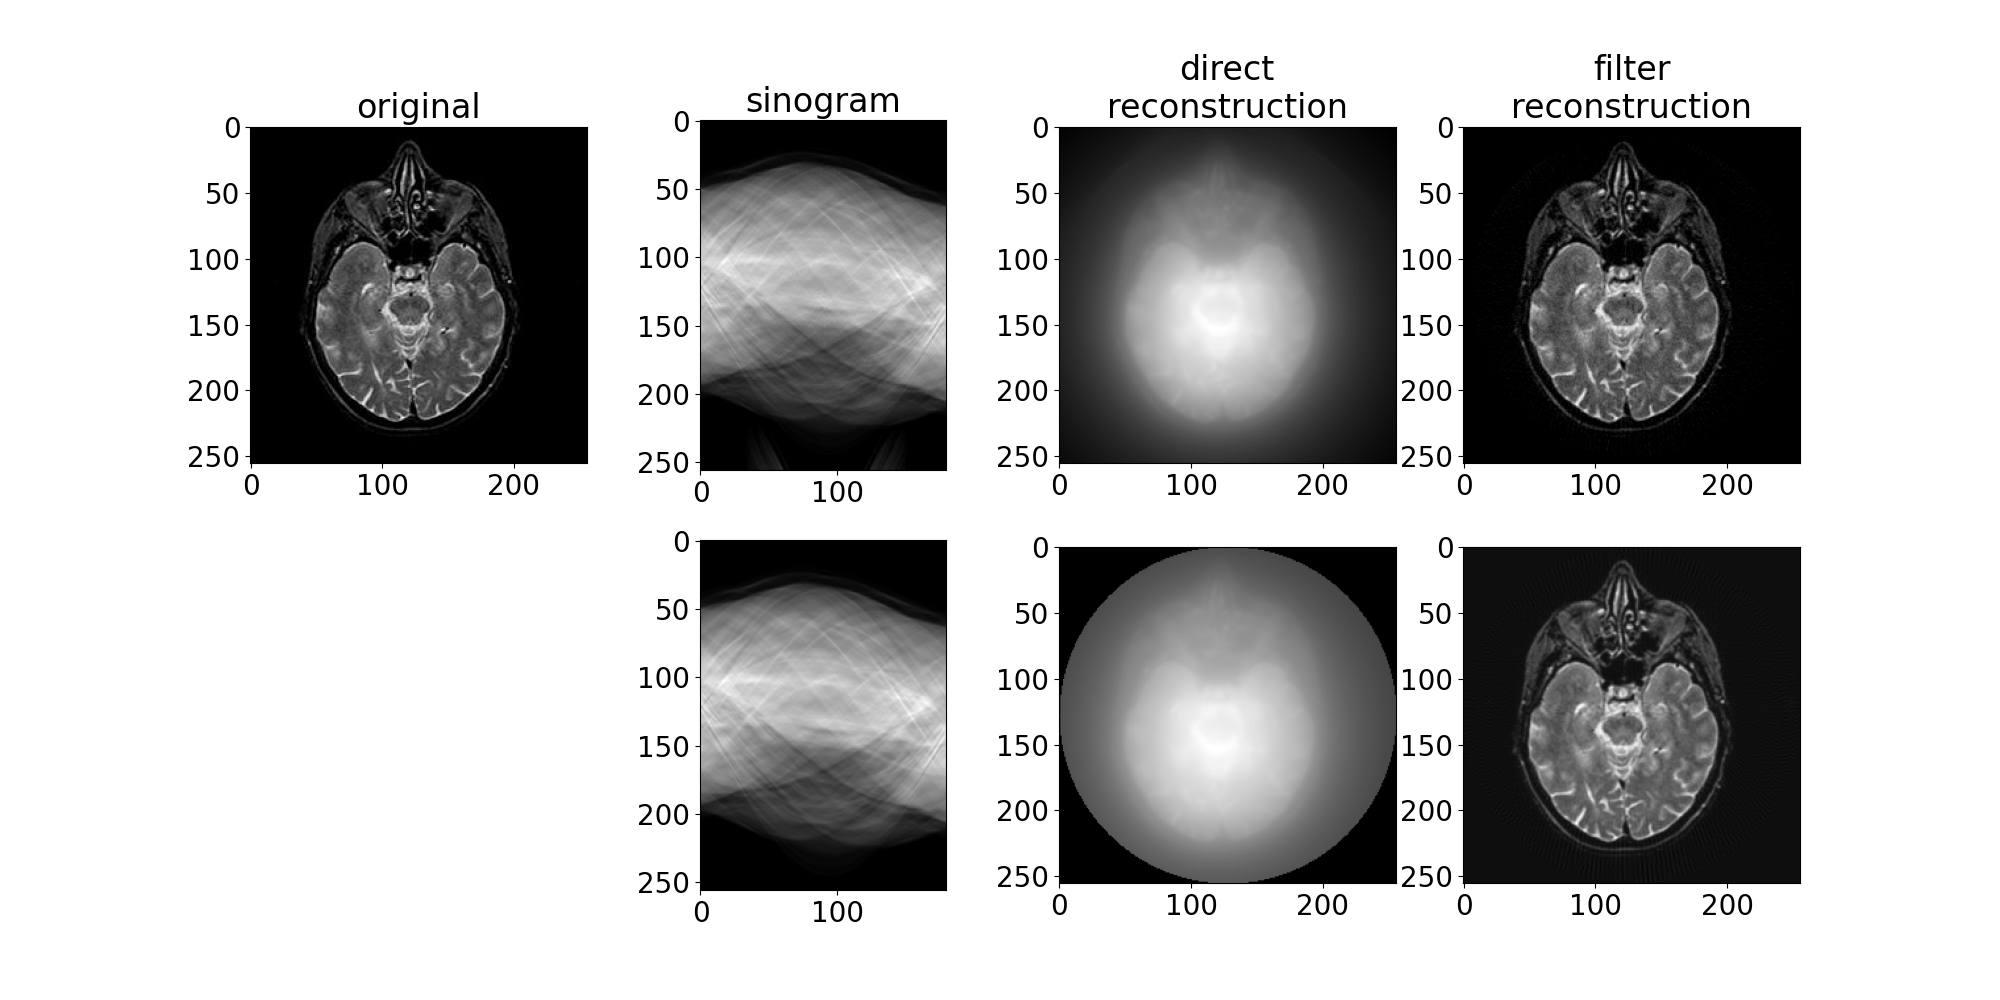
\includegraphics[width=0.9\textwidth]{../image/CT_result.png}
    \caption{CT图像重建结果}
    \label{fig result2}
\end{figure}
可以看到,无论是使用shepp-logan模型,还是使用一般的CT图像,本算法都取得了不错的效果,而且对于重建图像的周边部分进行了后处理,避免了skimage库算法中出现扫描区域边界重建之后颜色断层的结果。


\subsection{运算速度}
除了图像本身的质量以外,我还测试了本实现方法在不同图像大小情况下的运算速度,结果如下表\ref{tab:time_cost}
% Table generated by Excel2LaTeX from sheet 'time_cost'
\begin{table}[htbp]
    \centering
    \caption{算法速度对比(时间:秒)}
      \begin{tabular}{clrrr}
      \toprule
      \multicolumn{1}{l}{file} & method & \multicolumn{1}{l}{radon} & \multicolumn{1}{l}{iradon(direct)} & \multicolumn{1}{l}{iradon(filter)} \\
      \midrule
      \multirow{2}[0]{*}{res\textbackslash{}shepp-logan1024.jpg} & my algorithm & 15.82 & 17.22 & 17.09 \\
            & skimage & 8.53  & 5.84  & 5.82 \\
      \multirow{2}[0]{*}{res\textbackslash{}shepp-logan256.jpg} & my algorithm & 2.59  & 1     & 0.96 \\
            & skimage & 0.51  & 0.3   & 0.3 \\
      \multirow{2}[0]{*}{res\textbackslash{}shepp-logan512.jpg} & my algorithm & 5.95  & 4.08  & 4.18 \\
            & skimage & 2.07  & 1.44  & 1.61 \\
      \bottomrule
      \end{tabular}%
    \label{tab:time_cost}%
  \end{table}%
可以看到,算法的速度在可接受范围内,但是与优化过的第三方库相比还有一定的差距。
  
    
\section{感想与展望}

本次大作业我实现了一个简单的CT扫描和重建算法。并通过一些辅助代码进行了可视化和计时测试,完成了一个比较完整的流程。然而现在实现的算法还存在以下几点不足:
\begin{itemize}
    \item 运算速度相比第三方库的算法还有一定差距,需要进一步优化
    \item 只实现了平行束扫描和重建的方法,扫描速度较慢,没有涉及扇形束和锥形束。
    \item 对于异常值和结果的后处理部分比较简单粗暴,没有找到更好的解决方法。
\end{itemize}

最后,感谢助教和老师在本次大作业过程中给予的帮助。
\bibliographystyle{plain}
\bibliography{ref}

\end{document}
